\documentclass{article}

\usepackage[english]{babel}
\usepackage[utf8]{inputenc}
\usepackage{amsmath,amssymb}
\usepackage{parskip}
\usepackage{graphicx}

% Margins
\usepackage[top=2.5cm, left=3cm, right=3cm, bottom=4.0cm]{geometry}
% Colour table cells
\usepackage[table]{xcolor}

% Get larger line spacing in table
\newcommand{\tablespace}{\\[1.25mm]}
\newcommand\Tstrut{\rule{0pt}{2.6ex}}         % = `top' strut
\newcommand\tstrut{\rule{0pt}{2.0ex}}         % = `top' strut
\newcommand\Bstrut{\rule[-0.9ex]{0pt}{0pt}}   % = `bottom' strut

%%%%%%%%%%%%%%%%%
%     Title     %
%%%%%%%%%%%%%%%%%
\title{Coursework template CO343}
\author{Firstname Lastname \\ CID 01234567}
\date{\today}

\begin{document}
\maketitle

%%%%%%%%%%%%%%%%%
%   Problem 1   %
%%%%%%%%%%%%%%%%%
\section{Problem 1}
The problem states that we should find $x$ that solves the following equation
\begin{align}
    \label{eq:example_equation} % Equation label; can be used for referencing
    2 x^2 + 4 x - 6 = 0 \,.
\end{align}
We take the standard algorithm for solving equations of the form $a x^2 + bx + c$ and apply it to Equation~\ref{eq:example_equation}. This gives us
\begin{align}
    x 
    &= \frac{2}{2 \cdot 2} \pm \sqrt{\left( \frac{2}{2 \cdot 2} \right)^2 + \frac{6}{2} } \\
    &= 1 \pm 2
\end{align}
So the solutions are $x=3$ and $x = -1$.

% Example of how to add figure (can be used for jpeg, png, pdf, eps etc)
In Figure~\ref{fig:universe}, we can see an example of a galaxy.
\begin{figure}[h!]
    \centering
    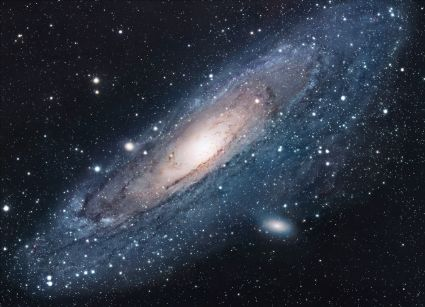
\includegraphics[scale=2]{universe.jpg}
    \caption{Example figure}
    \label{fig:universe}
\end{figure}


%%%%%%%%%%%%%%%%%
%   Problem 2   %
%%%%%%%%%%%%%%%%%
\pagebreak
\section{Problem 2}

Example of Simplex tableau:
\begin{align}
    \begin{array}{c | cccccc | c}
         BV  & z & x_1 & x_2 & x_3 & x_4 & x_5 & RHS \\ 
         \hline % horizontal line
         z   & 1 & 0 & 0 & -\tfrac{2}{5} & -\tfrac{1}{5} & 0 & -8 \\
         x_2 & 0 & 0 & 1 & -\tfrac{1}{5} & \tfrac{2}{5}  & 0 & 5 \\
         x_5 & 0 & 0 & 0 & -\tfrac{3}{5} & \tfrac{1}{5}  & 1 & 1 \\
         x_1 & 0 & 1 & 0 & \tfrac{3}{5}  & -\tfrac{1}{5} & 0 & 3
    \end{array}
\end{align}


We can define the \LaTeX{} commands \texttt{Tstrut} and \texttt{Bstrut} to get more spacing between rows in the tableau and make it look nicer:
\begin{align}
    \begin{array}{c | cccccc | c}
         BV  & z & x_1 & x_2 & x_3 & x_4 & x_5 & RHS \Tstrut\Bstrut \\ 
         \hline
         z   & 1 & 0 & 0 & -\tfrac{2}{5} & -\tfrac{1}{5} & 0 & -8 \Tstrut\Bstrut \\
         x_2 & 0 & 0 & 1 & -\tfrac{1}{5} & \tfrac{2}{5}  & 0 & 5  \Tstrut\Bstrut \\
         x_5 & 0 & 0 & 0 & -\tfrac{3}{5} & \tfrac{1}{5}  & 1 & 1  \Tstrut\Bstrut \\
         x_1 & 0 & 1 & 0 & \tfrac{3}{5}  & -\tfrac{1}{5} & 0 & 3  \Tstrut\Bstrut
    \end{array}
\end{align}

We can colour text and highlight cells in tableau, or just leave them empty:
\begin{align}
    \begin{array}{c | cccccc | c}
         BV  & z & x_1 & x_2 & x_3 & x_4 & x_5 & RHS \Tstrut\Bstrut \\ 
         \hline
         z   & 1 & & & -\tfrac{2}{5} & -\tfrac{1}{5} & & -8 \Tstrut\Bstrut \\
         x_2 & & & \cellcolor{gray!50}1 & -\tfrac{1}{5} & \tfrac{2}{5} & & 5 \Tstrut\Bstrut \\
         x_5 & & & & -\tfrac{3}{5} & \tfrac{1}{5}  & 1 & 1 \Tstrut\Bstrut \\
         x_1 & & \textcolor{red}{1} & & \tfrac{3}{5}  & -\tfrac{1}{5} & & 3 \Tstrut\Bstrut
    \end{array}
\end{align}

Here is how you make vectors and matrices:
\begin{align}
    \mathbf x = \begin{bmatrix} 1 & 2 & 3 \end{bmatrix} = \begin{bmatrix} 1 \\ 2 \\ 3 \end{bmatrix}^\top \\
    \mathbf A = \begin{bmatrix} 1 & 2 & 3 \\ 4 & 5 & 6 \end{bmatrix}^{-1}
\end{align}

Here is a formulation of a linear program:
\begin{align*}
    \min_{x} \quad & c^\top x \\
    \mathrm{s.t.} \quad 
    & A x \leq b \\
    &-1 \leq x_n \leq 1 \,, \quad n = 1, \dots, N
\end{align*}

There is an ocean of Latex questions and answers online. If you have a question, most likely someone else will have asked the same question before. 

\end{document}
